Multiple choice section. All points are for choosing the correct answer. No justification is needed.
\begin{questions} 

\question[2] Select the function graphed below.

\begin{multicols}{2}
    

    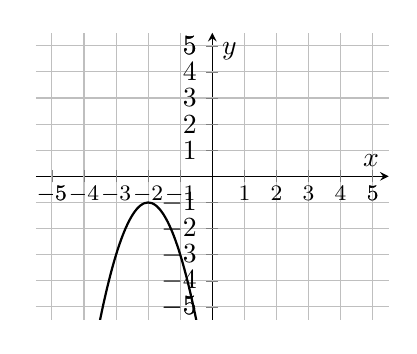
\begin{tikzpicture}
\begin{axis}[
   grid = major,
   extra x ticks={-6,-5,-4,-3,-2,-1,1,2,3,4,5,6},
   extra y ticks={-6,-5,-4,-3,-2,-1,1,2,3,4,5,6},
   %ytick= false,
   %xminorgrids=true,
   width=.5\textwidth,
   %clip = true,
   %clip mode=individual,
   %restrict y to domain=-12:12,
   axis x line = middle,
   axis y line = middle,
   %     yticklabel style = {font=\footnotesize,xshift=0.5ex},
        xticklabel style = {font=\footnotesize,yshift=0.5ex},
   xlabel={$x$},
   %xlabel style={at=(current axis.right of origin)},
   ylabel={$y$},
   %ylabel style={at=(current axis.above origin)},
   %domain = -5:5,
   xmin = -5,
   xmax = 5,
   enlarge y limits={rel=0.05},
   enlarge x limits={rel=0.05},
   ymin = -5,
   ymax = 5,
 ]
\addplot[smooth, thick, domain = -4:0,samples=35
	] { -2*(x+2)^2-1};
% \addplot[smooth, thick, domain = 1.15:6.5,
%	] { (3*x^2+5*x-2)/(x-1)};
\end{axis}
\end{tikzpicture}
\begin{checkboxes}
    \choice $f(x)=-2(x+2)^2-1$
    \choice $f(x)=2(x+2)^2+1$
    \choice $f(x)=-2(x-2)^2-1$
    \choice $f(x)=-2(x-2)^2+1$
    \choice None of the above.
\end{checkboxes}
\end{multicols}
\question[2] Determine which rational function could generate the graph below.

\begin{multicols}{2}
    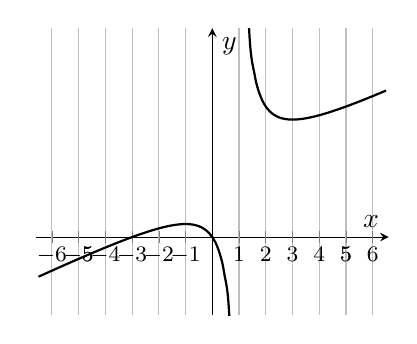
\begin{tikzpicture}
\begin{axis}[
   grid = major,
   extra x ticks={-6,-5,-4,-3,-2,-1,1,2,3,4,5,6},
   %extra y ticks={-6,-5,-4,-3,-2,-1,1,2,3,4,5,6},
   ytick= false,
   %xminorgrids=true,
   width=.5\textwidth,
   %clip = true,
   %clip mode=individual,
   %restrict y to domain=-12:12,
   axis x line = middle,
   axis y line = middle,
   %     yticklabel style = {font=\footnotesize,xshift=0.5ex},
        xticklabel style = {font=\footnotesize,yshift=0.5ex},
   xlabel={$x$},
   %xlabel style={at=(current axis.right of origin)},
   ylabel={$y$},
   %ylabel style={at=(current axis.above origin)},
   %domain = -5:5,
   xmin = -6,
   xmax = 6,
   enlarge y limits={rel=0.05},
   enlarge x limits={rel=0.05},
   ymin = -5,
   ymax = 15,
 ]
\addplot[smooth, thick, domain = -6.5:0.87,samples=35
	] { (x^2+3*x)/(x-1)};
 \addplot[smooth, thick, domain = 1.15:6.5,
	] { (x^2+3*x)/(x-1)};
\end{axis}
\end{tikzpicture}

%\begin{multicols}{2}
    
\begin{checkboxes}
    \choice $\dfrac{x^2-3x}{x-1}$
    \choice $\dfrac{x^2+3x}{x-1}$
    \choice $\dfrac{x^2+3x}{x^2-1}$
    \choice $\dfrac{x^2+3x}{x^3-1}$
    \choice None of the above.
\end{checkboxes}
\end{multicols}

\question[2] Solve the following inequality.
\[
2(3x-5)\geq 10
\]
\begin{checkboxes}
    \choice $\left(-\infty,\dfrac{10}{3}\right]$
    \choice $\left[\dfrac{10}{3},\infty\right)$
    \choice $\left(-\infty,\dfrac{10}{3}\right)$
    \choice $\left(\dfrac{10}{3},\infty\right)$
    \choice None of the above.
\end{checkboxes}
\newpage

\question[2] Consider quadratic, $f(x)=ax^2+bx+c$. What are we guaranteed about the zeros (roots) of the quadratic.
\begin{checkboxes}
    \choice $f(x)$ will have two integer roots (not necessarily distinct).
    \choice $f(x)$ will have two rational roots (not necessarily distinct).
    \choice $f(x)$ will have two real roots (not necessarily distinct).
    \choice $f(x)$ is not guaranteed to have any real roots.
    %\choice None of the above.
\end{checkboxes}

\question[2] Select the graph below that is not a function.
\begin{multicols}{2}
    

\begin{checkboxes}
    \choice \phantom{a}\vspace{-.7cm}
    
    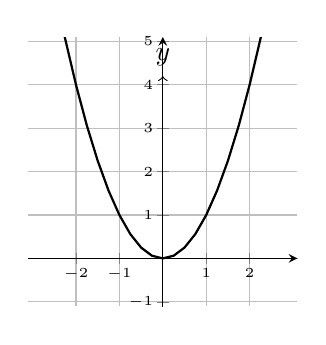
\begin{tikzpicture}%[domain=-4:4]
    \begin{axis}[
    grid=major,
    axis x line = middle,
    axis y line = middle,
        yticklabel style = {font=\tiny,xshift=0.5ex},
        xticklabel style = {font=\tiny,yshift=0.5ex},
    %scale only axis=true,
    width=5 cm,
    height=5 cm,
    xtick={-2,-1,0,1,2},
    ytick={-2,-1,0,1,2,3,4,5},
    xmin=-3.1,
    xmax=3.1,
    ymin=-1.1,
    ymax=5.1,
    ]
  %\draw[very thin,color=gray] (-2.9,-2.1) grid (2.9,2.9);

  \draw[->] (-4.2,0) -- (4.2,0) node[right] {$x$};
  \draw[->] (0,-1.2) -- (0,4.2) node[above] {$y$};

  \draw[thick, domain=-3:3]    plot (\x,\x*\x) ;%            node[right] {$f(x) =x$};
  % \x r means to convert '\x' from degrees to _r_adians:
  %\draw[thick, domain=-1:2]   plot (\x,2*\x) ;%   node[right] {$f(x) = \sin x$};
  %\draw[color=orange] plot (\x,{0.05*exp(\x)}) node[right] {$f(x) = \frac{1}{20} \mathrm e^x$};
  \end{axis}
\end{tikzpicture}

\choice \phantom{b}\vspace{-.7cm}
    
    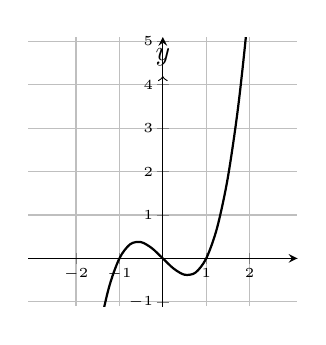
\begin{tikzpicture}%[domain=-4:4]
    \begin{axis}[
    grid=major,
    axis x line = middle,
    axis y line = middle,
        yticklabel style = {font=\tiny,xshift=0.5ex},
        xticklabel style = {font=\tiny,yshift=0.5ex},
    %scale only axis=true,
    width=5 cm,
    height=5 cm,
    xtick={-2,-1,0,1,2},
    ytick={-2,-1,0,1,2,3,4,5},
    xmin=-3.1,
    xmax=3.1,
    ymin=-1.1,
    ymax=5.1,
    ]
  %\draw[very thin,color=gray] (-2.9,-2.1) grid (2.9,2.9);

  \draw[->] (-4.2,0) -- (4.2,0) node[right] {$x$};
  \draw[->] (0,-1.2) -- (0,4.2) node[above] {$y$};

  \draw[thick, smooth, domain=-3:3]    plot (\x,\x*\x*\x-\x) ;%            node[right] {$f(x) =x$};
  % \x r means to convert '\x' from degrees to _r_adians:
  %\draw[thick, domain=-1:2]   plot (\x,2*\x) ;%   node[right] {$f(x) = \sin x$};
  %\draw[color=orange] plot (\x,{0.05*exp(\x)}) node[right] {$f(x) = \frac{1}{20} \mathrm e^x$};
  \end{axis}
\end{tikzpicture}

\choice \phantom{c}\vspace{-.7cm}
    
    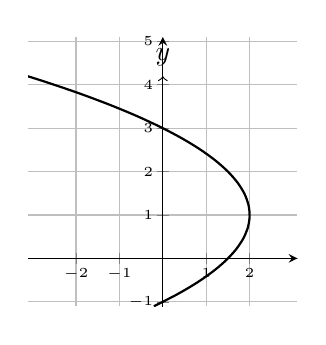
\begin{tikzpicture}%[domain=-4:4]
    \begin{axis}[
    grid=major,
    axis x line = middle,
    axis y line = middle,
        yticklabel style = {font=\tiny,xshift=0.5ex},
        xticklabel style = {font=\tiny,yshift=0.5ex},
    %scale only axis=true,
    width=5 cm,
    height=5 cm,
    xtick={-2,-1,0,1,2},
    ytick={-2,-1,0,1,2,3,4,5},
    xmin=-3.1,
    xmax=3.1,
    ymin=-1.1,
    ymax=5.1,
    ]
  %\draw[very thin,color=gray] (-2.9,-2.1) grid (2.9,2.9);

  \draw[->] (-4.2,0) -- (4.2,0) node[right] {$x$};
  \draw[->] (0,-1.2) -- (0,4.2) node[above] {$y$};

\draw[thick]
plot[variable=\t,domain=-2.1:4.1,smooth,thick] (-0.5*\t*\t+2,\t+1);
  %\draw[thick, domain=-3:3]    plot (\x,1+.25*2^\x) ;%            node[right] {$f(x) =x$};
  % \x r means to convert '\x' from degrees to _r_adians:
  %\draw[thick, domain=-1:2]   plot (\x,2*\x) ;%   node[right] {$f(x) = \sin x$};
  %\draw[color=orange] plot (\x,{0.05*exp(\x)}) node[right] {$f(x) = \frac{1}{20} \mathrm e^x$};
  \end{axis}
\end{tikzpicture}

\choice \phantom{d}\vspace{-.7cm}
    
    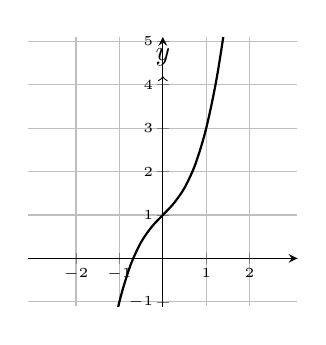
\begin{tikzpicture}%[domain=-4:4]
    \begin{axis}[
    grid=major,
    axis x line = middle,
    axis y line = middle,
        yticklabel style = {font=\tiny,xshift=0.5ex},
        xticklabel style = {font=\tiny,yshift=0.5ex},
    %scale only axis=true,
    width=5 cm,
    height=5 cm,
    xtick={-2,-1,0,1,2},
    ytick={-2,-1,0,1,2,3,4,5},
    xmin=-3.1,
    xmax=3.1,
    ymin=-1.1,
    ymax=5.1,
    ]
  %\draw[very thin,color=gray] (-2.9,-2.1) grid (2.9,2.9);

  \draw[->] (-4.2,0) -- (4.2,0) node[right] {$x$};
  \draw[->] (0,-1.2) -- (0,4.2) node[above] {$y$};

  \draw[thick, smooth, domain=-3:3]    plot (\x,\x*\x*\x+\x+1) ;%            node[right] {$f(x) =x$};
  % \x r means to convert '\x' from degrees to _r_adians:
  %\draw[thick, domain=-1:2]   plot (\x,2*\x) ;%   node[right] {$f(x) = \sin x$};
  %\draw[color=orange] plot (\x,{0.05*exp(\x)}) node[right] {$f(x) = \frac{1}{20} \mathrm e^x$};
  \end{axis}
\end{tikzpicture}

\end{checkboxes}
\end{multicols}

\question[2] Find all solutions to the following equation.
    \[ x^3=x\]
\begin{checkboxes}
%\choice $x=1$
    \choice $x=1$, $x=0$
    \choice $x=1$, $x=-1$
    \choice $x=1$, $x=-1$, $x=0$
    \choice $x=i$, $x=-i$, $x=1$
    \choice None of the above.
\end{checkboxes}

%\question[2] 
%\begin{checkboxes}
%    \choice 1
%    \choice 2
%    \choice 3
%    \choice 4
%    \choice None of the above.
%\end{checkboxes}
\newpage
\hspace{-.5in}Free answer section. Work must be shown to get credit for any answer. Partial credit may be given even for incorrect final answers, so show your work.
%\question[10] b

\question[5] Solve the following inequality.
\[
2|3-x|\geq 1
\]

\vspace{12cm}

\question[5] Write a polynomial, $P(x)$ with roots of $-3$, $6$, a repeated root at $11$ with multiplicity 3, and as $x\to -\infty$, $P(x)\to +\infty$ and as $x\to +\infty$, $P(x)\to -\infty$

\newpage
\question %\textbf{[Section 1.4-1.5, 2.7, 3.4]} 
Let $f(x) = x^2 - x - 20$.
%Let $f(x) = x^2 - 3x - 10$ and $g(x) = x^2$.

\begin{parts}
    \part[3] Find all the roots of $f(x)$. \vspace{4cm}
    
    \part[3] Let $g(x) = x^2$, find $(f \circ g)(x)$.
    \vspace{4cm}

    \part[3] What are all the possible \textbf{rational roots} of $(f \circ g)(x)$ according to the \textbf{rational root theorem}?
    \vspace{4cm}

    \part[1] Using Part (a) of the question, find all the \textbf{roots} of $(f \circ g)(x)$. Credit will be given solely based on whether the answer is correct. (\textbf{Hint}: Some of the roots are complex numbers).
\end{parts}

\newpage

\question[5] %\textbf{[Section 4.3, 4.4]} 
%\begin{parts}
    %\part[5] 
    Expand the following log function with no interior multiplications or divisions and simplified powers as much as the log rules allow
    \[\ln \frac{x^3y}{\sqrt{x-y}}.\]
    \vspace{5cm}

    %\part[5] Rewrite the following logarithmic expressions as a single logarithm
%    \[x\log_7(4+x) + \log_7 y - z\log_7 w. \]
%\end{parts}

\question[5] Perform the following operation and write as a single fraction.
\[
\frac{x}{x+2}+\frac{x-3}{x^2+7x+10}
\]

\newpage
\question %\textbf{[Section 4.1, 4.2, (and a bit of 4.5 involved)]} 
Let $f(x)=\log_2(3-x)$.
\begin{parts}
    \part[3] Find the domain of $f(x)$.
    \vspace{4cm}
    \part[3] Find the zero of $f(x)$
    \vspace{4cm}
    %\part[2] Find the vertical asymptote of  $f(x)$.
    %\vspace{2cm}
    \part[4] Compute the inverse function $f^{-1}(x)$.
\end{parts}

\newpage


\question %\textbf{[Section 5.1]}
For each of the following systems of linear equations, determine whether or not the system has any solutions. For the systems that have solutions, find all solutions; for the systems that have infinitely many solutions, write your solutions as an ordered pair in terms of the variable $x$ only.

\begin{parts}
    
    % \part[4]
    % \begin{align*}
    %     x - 3y &= 1 \\
    %     -2x + 6y &= 3 
    % \end{align*}
    % \vspace{2in}
    
    \part[4] 
    \begin{align*}
        5 x  -  y &= 5 \\
          x  +  3y &= -7
    \end{align*}
    %\vspace{2in}
    \vfill
    \part[4]
    \begin{align*}
        2x - 2y &= 3 \\
        -4x + 4y &= -6
    \end{align*}
    \vfill
\end{parts}



\newpage
\question %\textbf{[Section 3.7]}
Consider the rational function \[f(x)=\frac{2x+5}{x^2+2x-35}\]
\begin{parts}
    \part[2] Find the zeroes of $f$.
    \vspace{4cm}
    \part[2] Find the vertical asymptotes of $f$.
    \vspace{4cm}
    \part[5] Solve the following inequality and put your final answers in interval notation.\[\frac{2x+5}{x^2+2x-35}\geq 0\]
\end{parts}

\newpage
\question[10] %\textbf{[Section 5.2]}
Find the complete solution of the linear system, or show that it has no solution.
\begin{equation*}
    \left\{
    \begin{aligned}
         x+y+z&=1\\
        2x-y-2z&=0\\
        5x-3y-6z&=10\\
    \end{aligned}\right.
\end{equation*}

\newpage

\question[6] %\textbf{[Section 2.1-2.2]}
Find the domain of the function 

\begin{equation*}
    f(x) = \sqrt{2+x} + \dfrac{1}{\sqrt{2-x}}
\end{equation*}
\vspace{8cm}

\question[6]
Find the solution(s) to the following equation.
\[
\log_2(x+7)+\log_2(x)=3
\]


\newpage
\question[5] %\textbf{[Section 4.4-4.5]}
This problem involves the radioactive decay model, $A(t)=A_, e^{-kt}$

You may have heard of radiocarbon dating, in which the age of materials can be estimated by measuring how much Carbon-14 they contain.  
%The half-life of Carbon-14 is about 5730 years.

%Suppose a scroll is discovered at a dig in Pompeii.  Assume the scroll 
Assume a sample originally had 14 pg (picograms) of Carbon-14. The same sample has 7 pg of Carbon-14 after 5730 years.

%\begin{parts}
%    \part[5] 
    Find the value of $k$ in the radioactive decay model. (Leave it in terms of a log.)% Write a function which describes the amount of Carbon-14 remaining in the scroll $t$ years after it was created.

    \vspace{.35\textheight}
    
    \question[5] A population of 20 cats is sent to a  moon habitat and the population begins to grow. The number of moon-cats is modelled by $n(t)=P_0 e^{0.21t}$, with $t$ measured in years.

    How many years will it take for there to be 5000 moon-cats?
    %Today, the scroll is measured to contain 10.6 pg of Carbon-14.  Using your function from part (a), write an expression for the age of the scroll. [Solve for $t$.] \\
    (Leave your answer in terms of a log.)
%\end{parts}

\end{questions}